\documentclass[pdf]{beamer}
\usepackage{algorithmic,algorithm}
\usepackage{amsmath}
\usepackage{graphicx}
\usepackage[T1]{fontenc}
\usepackage{bookmark}
\usepackage{array,booktabs}
\usepackage{lmodern}
\usepackage{textcomp}
%\usepackage{lmodern}
\usepackage{algorithmic,algorithm}
\usepackage{amssymb}
\renewcommand{\familydefault}{\sfdefault}
\usepackage{tocvsec2}
\setlength\parindent{0pt}
\setlength{\parskip}{1em}
\usepackage{xcolor}
\hbadness=10000
\hfuzz=50pt
\title{Theme : Machine learning for high energy physics (HEP)}
\subtitle{Dissertation Title : A meta-algorithm for cascades : A high energy physics application}
\author{Vidhi Lalchand\\
Supervisor: Dr. Anita Faul\\
Physics Advisor: Dr. Chris Lester}
\date{May 18, 2016}

\usetheme{CambridgeUK}

\begin{document}

\begin{frame}
\titlepage
\end{frame}

{
\usebackgroundtemplate{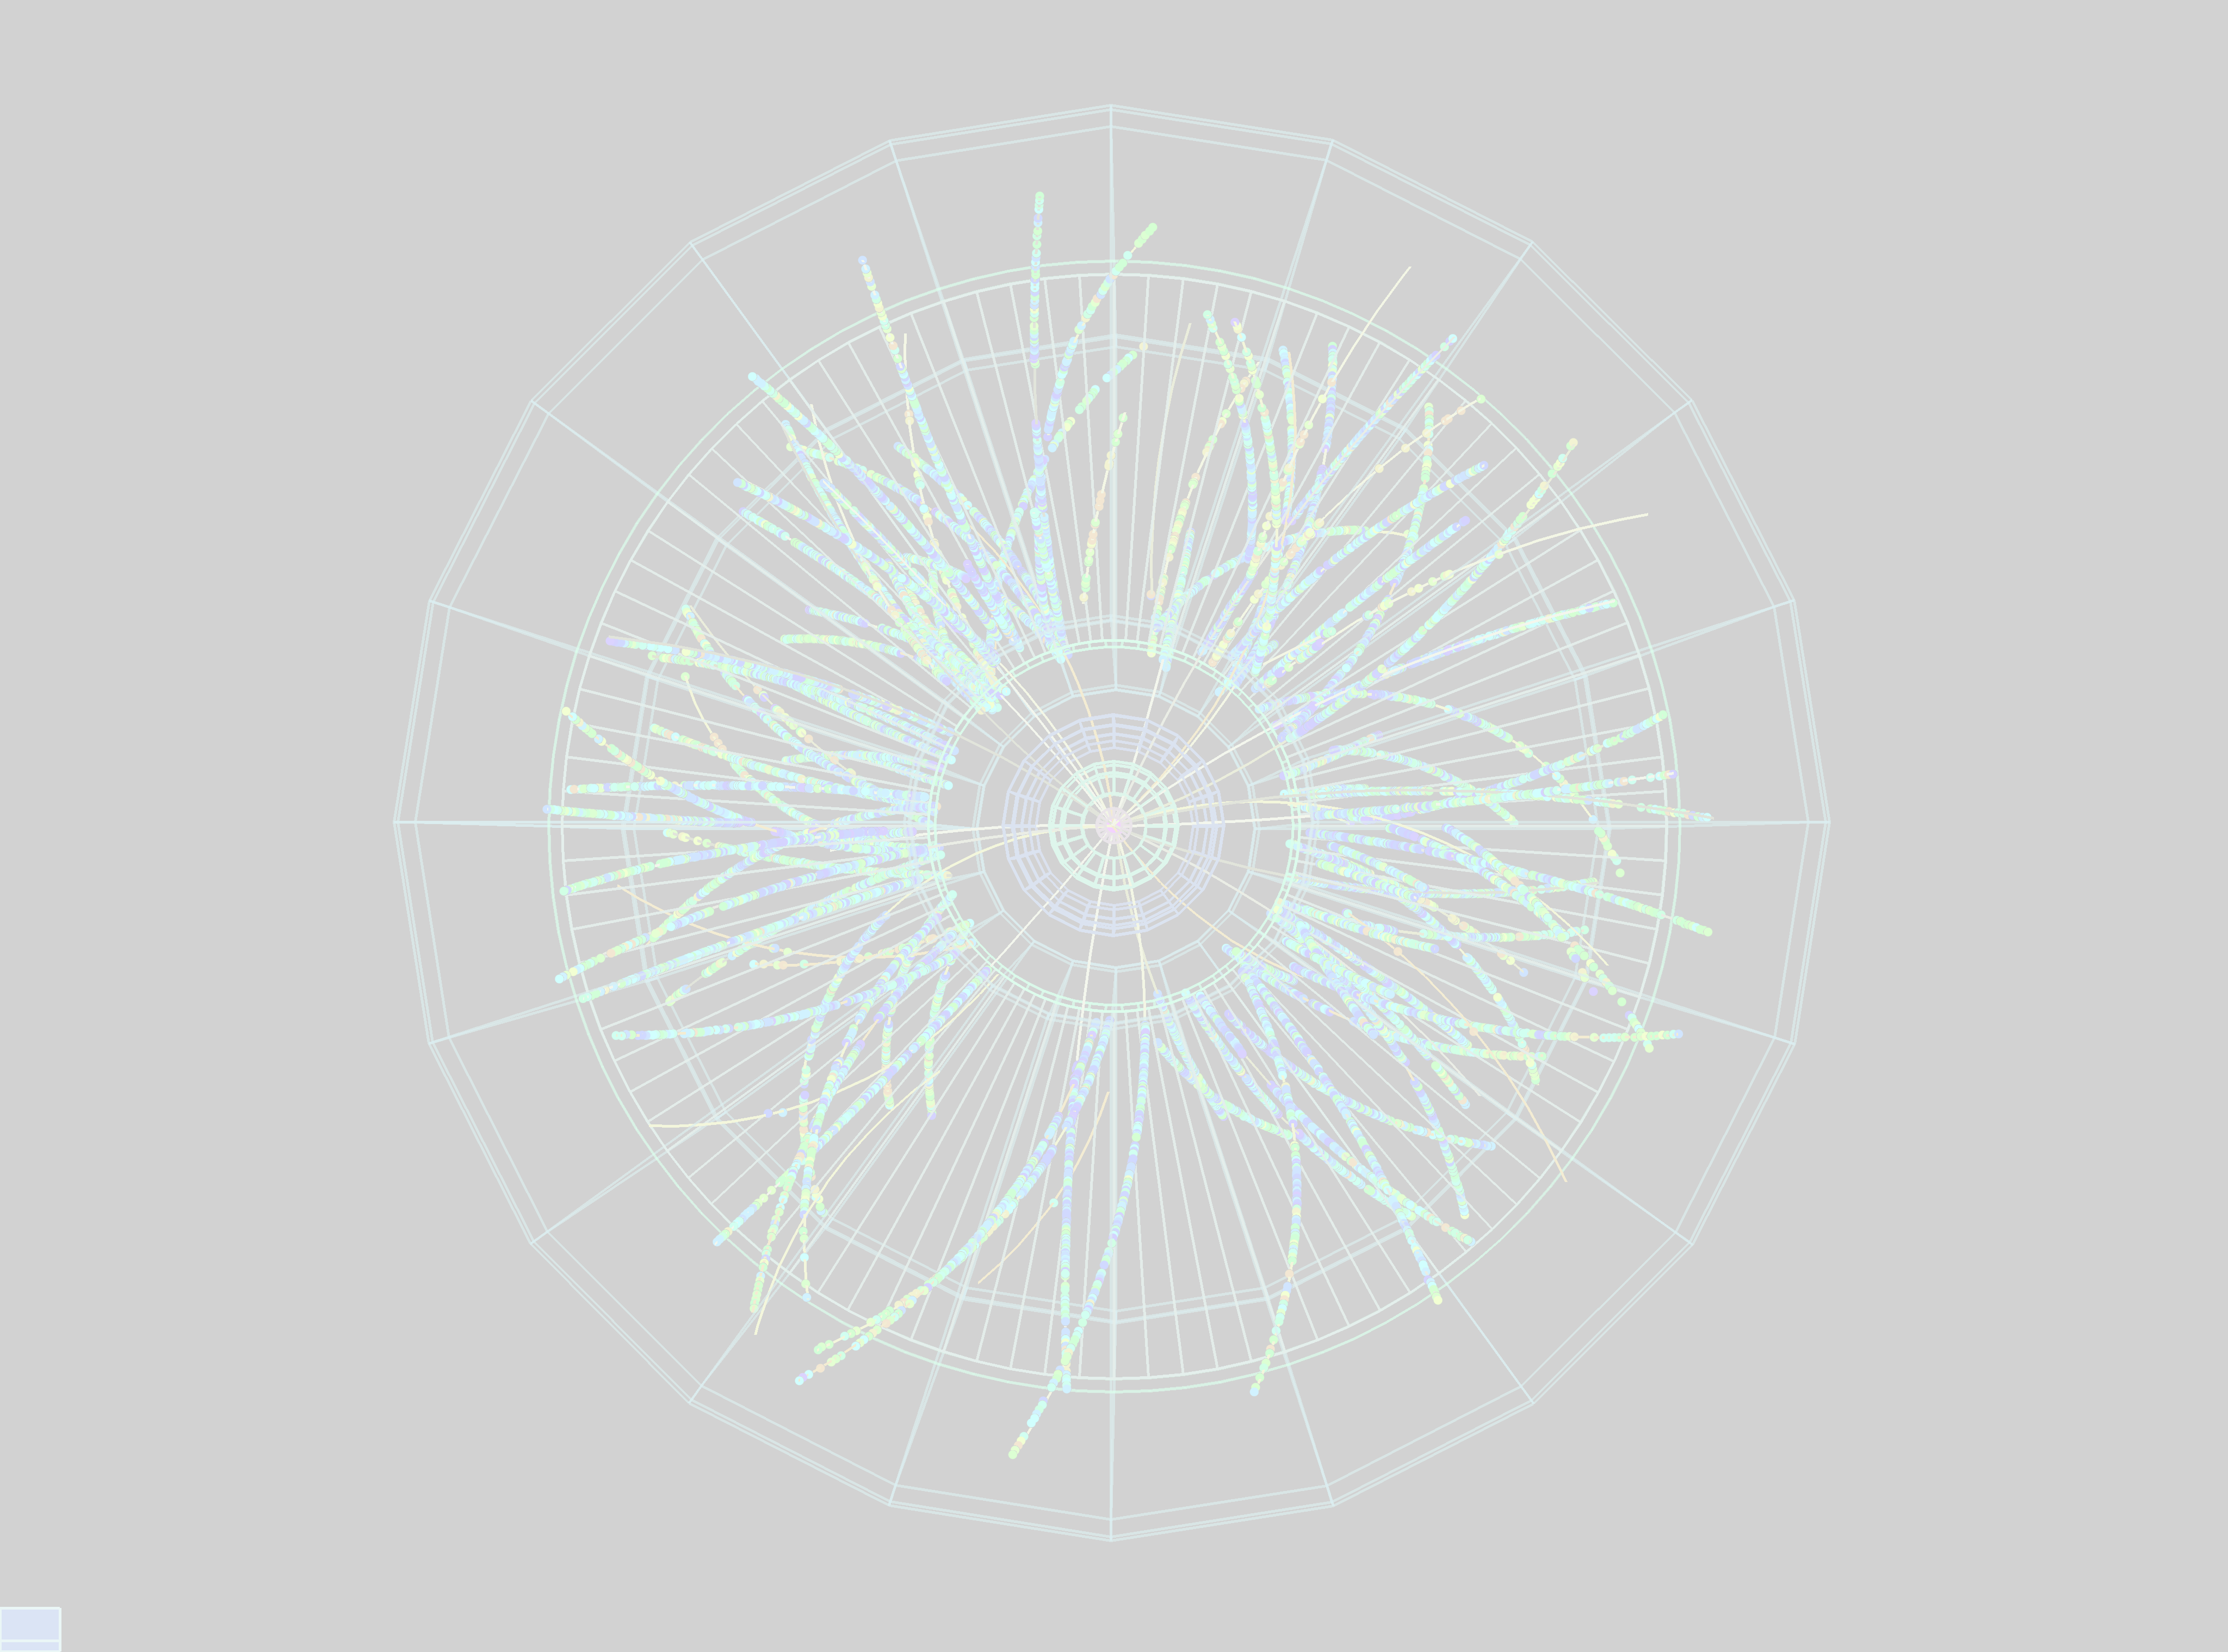
\includegraphics[width=\paperwidth]{front.png}}
\begin{frame}
\frametitle{The future of HEP}
\textcolor{cambridgedarkorange}{
\textit{`The future of high energy physics lies in large circular colliders colliding particles at really high energies'} - Nima Arkani Hamed.}\\
\bigskip
An important goal of the particle physics community worldwide is the search for new particles and physical processes that complement and go beyond the Standard Model of particle physics. Eg. Supersymmetry, the Higgs boson.
As the LHC is set to hit higher energy frontiers the rate of data collection is set to increase by a factor of 10.
\end{frame}
}

\begin{frame}
\frametitle{The process of discovery in HEP}
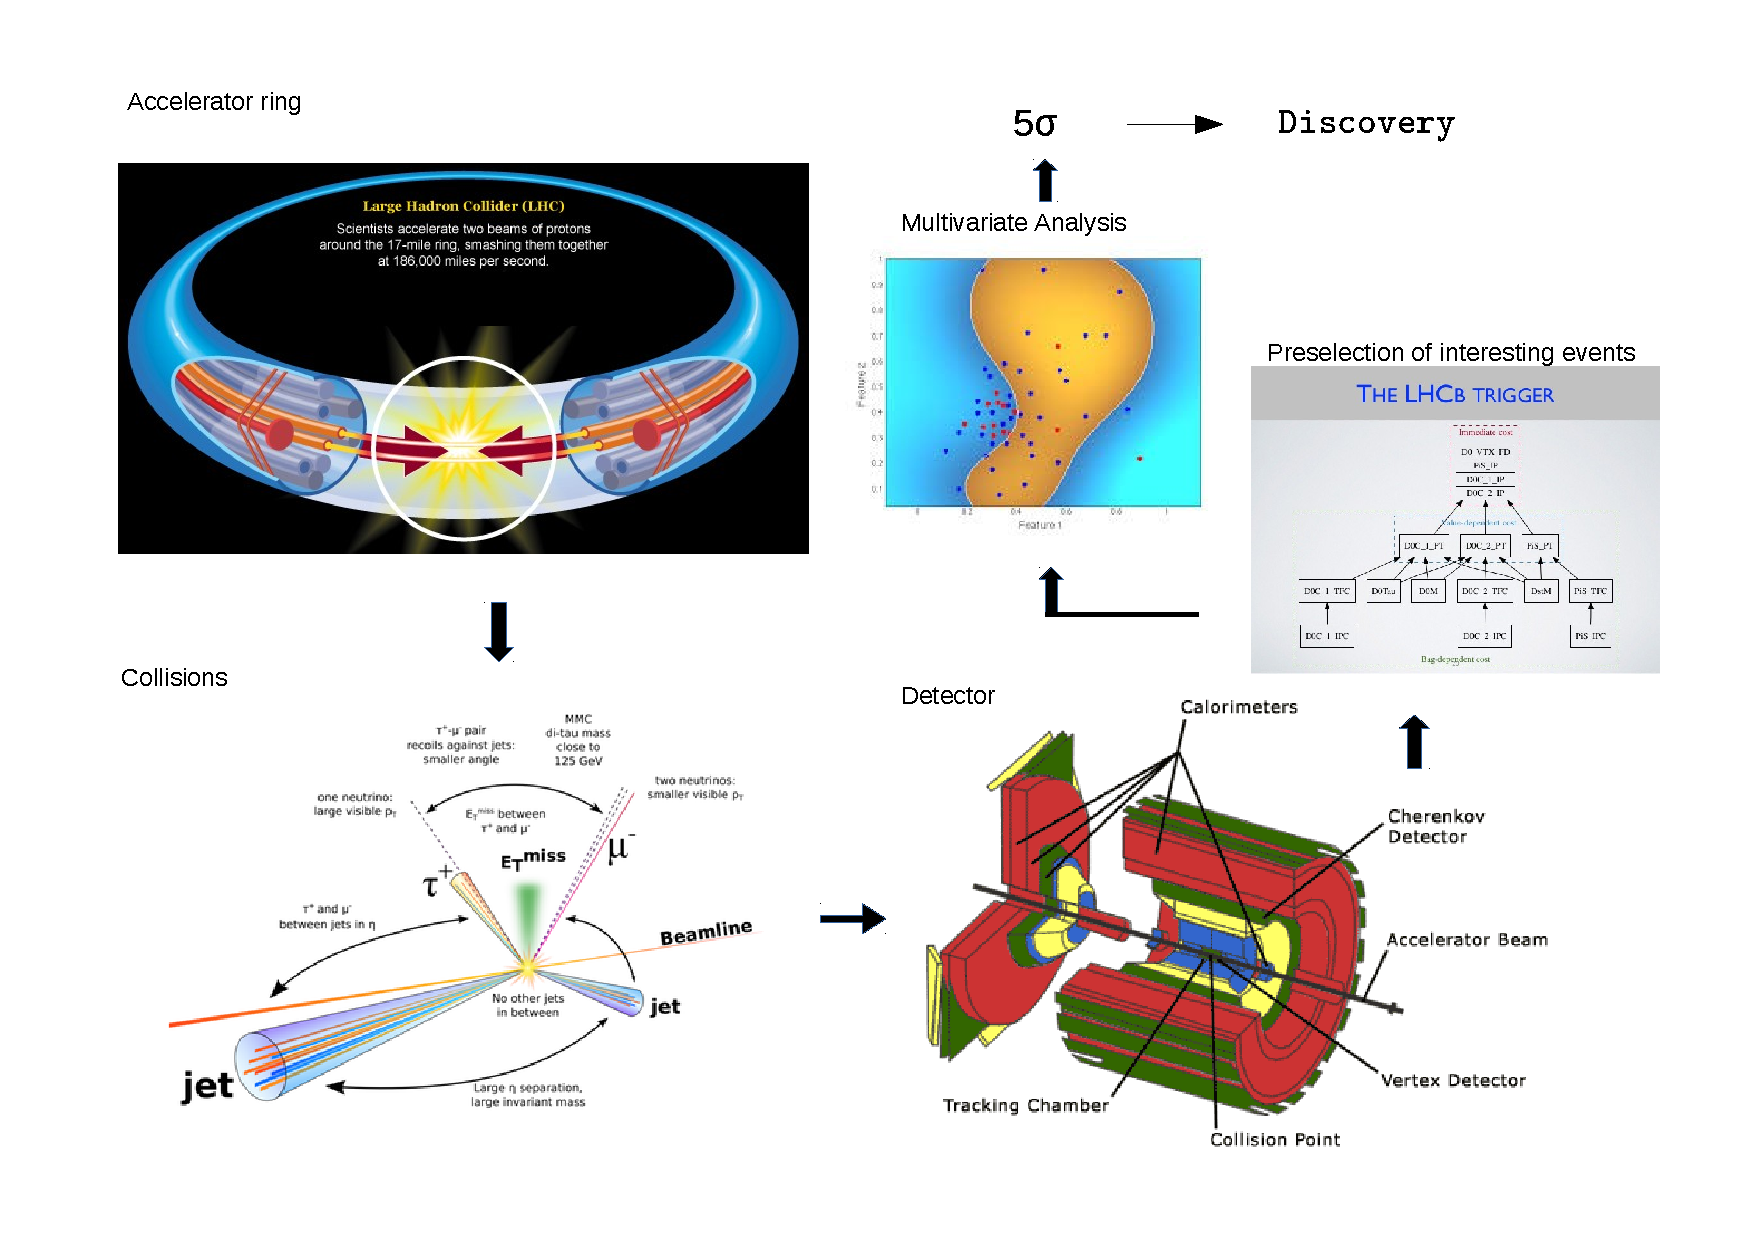
\includegraphics[scale=0.4]{discovery.pdf}
\end{frame}

\begin{frame}
\frametitle{Classification in HEP}
There are 3 types of classification processes that take place at the LHC. 
\begin{itemize}
\item<1->Trigger classifiers - fast and sclalable, real time signal/background separation. 
\item<2->  \textbf{Classification for discovery} - sophisticated models for signal/background separation which are slower to train and must learn to classify events from classes that mimic each other closely.  
\item<3-> Deep learning - Unsupervised learning, automatically inferring powerful latent features in the data. 
\end{itemize}

\end{frame}

\begin{frame}
\frametitle{Classification for discovery} 
Events generated in the collider are preprocessed and represented 
as high dimensional \textit{feature  vectors}. These can be represented as $ x \in \mathbb{R}^{d}$. 
A classifier $h(x): \mathbb{R}^d \rightarrow \mathbb{R}$ is trained to classify signal events (s) from background (b). It outputs a discriminant score taking small values in one class and large values in the other. By putting a threshold on the discriminant value, a selection region $\mathcal{H}$ is chosen.
\begin{center}
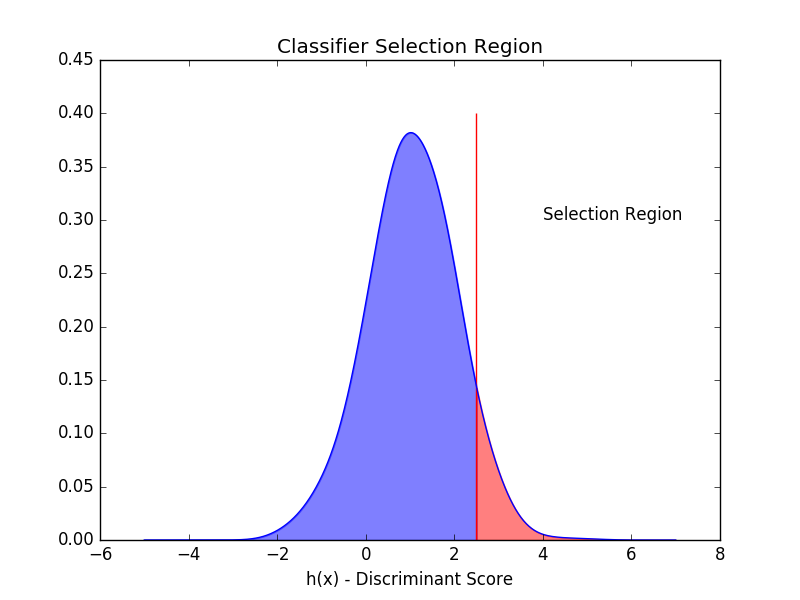
\includegraphics[scale=0.30]{selection_region.png}
\end{center}
\end{frame}

\begin{frame}
\frametitle{Classification for discovery - the math} 
Let the selection region $\mathcal{H}$ be characterized by,
\begin{equation}
\mathcal{H} = \{\textbf{x} : h(\textbf{x}) > \theta \}
\end{equation}
$s$: signal events in $\mathcal{H}$, or the true positives.\\
$b$: background events in $\mathcal{H}$, or the true negatives.\\
\begin{center}
AMS = $\dfrac{s}{\sqrt{b}}$ 
\end{center}
This is the fundamental objective function the classifiers are tuned to maximise. 
\end{frame}

\begin{frame}
\frametitle{Classification for discovery - the math}

The occurrence of background events follow a Poisson process. 
Over a given time period during which events are recorded, the expected number of \textit{selected} background events is $\mu_{b}$ and its variance is also $\mu_{b}$ 
The normalized statistic, 
\begin{equation} \hat{t} = (n-\mu_{b})/\sqrt{\mu_{b}} \sim N(0,1) 
\end{equation} serves as a test statistic for detection of signal events. A fluctuation is considered sufficiently large to claim a discovery of the signal process if it exceeds $5\sigma$, i.e. if $\hat{t} > 5$ ($\sigma = 1$ for the normalized test statistic).

\begin{equation}
(n-\mu_{b})/\sqrt{\mu_{b}} = ( s + b - b)/\sqrt{b} = s/\sqrt{b}
\end{equation}

\end{frame}

\begin{frame}
\frametitle{The Higgs particle (H)}
In 2012, the ATLAS experiment claimed the discovery of a new particle, the Higgs boson. The existence of this particle provides support to the theory that that a field permeates the universe through which fundamental particles acquire mass, a theory which is cardinal for the completeness of the Standard Model of particle physics.\\
\begin{center}
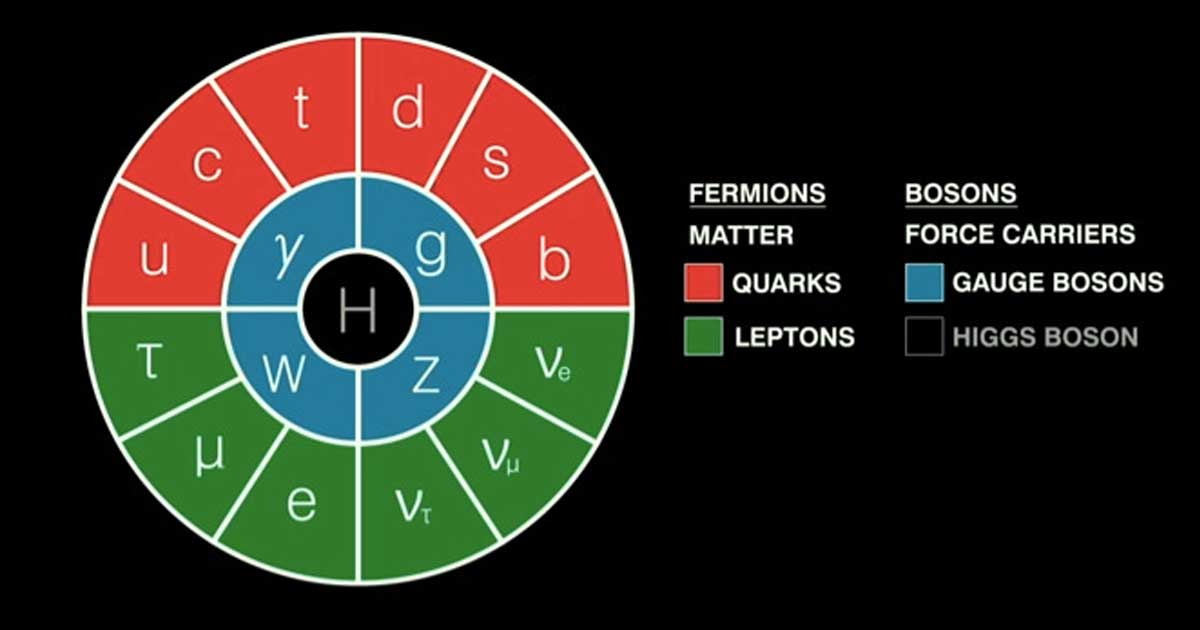
\includegraphics[scale=0.2]{standard_model.jpg}
\end{center}
\end{frame}

\begin{frame}
\frametitle{The Higgs Decay}
A key property of a particle is how it decays into other particles. The Higgs has 5 experimentally accessible decay channels.
\hspace*{-3mm}
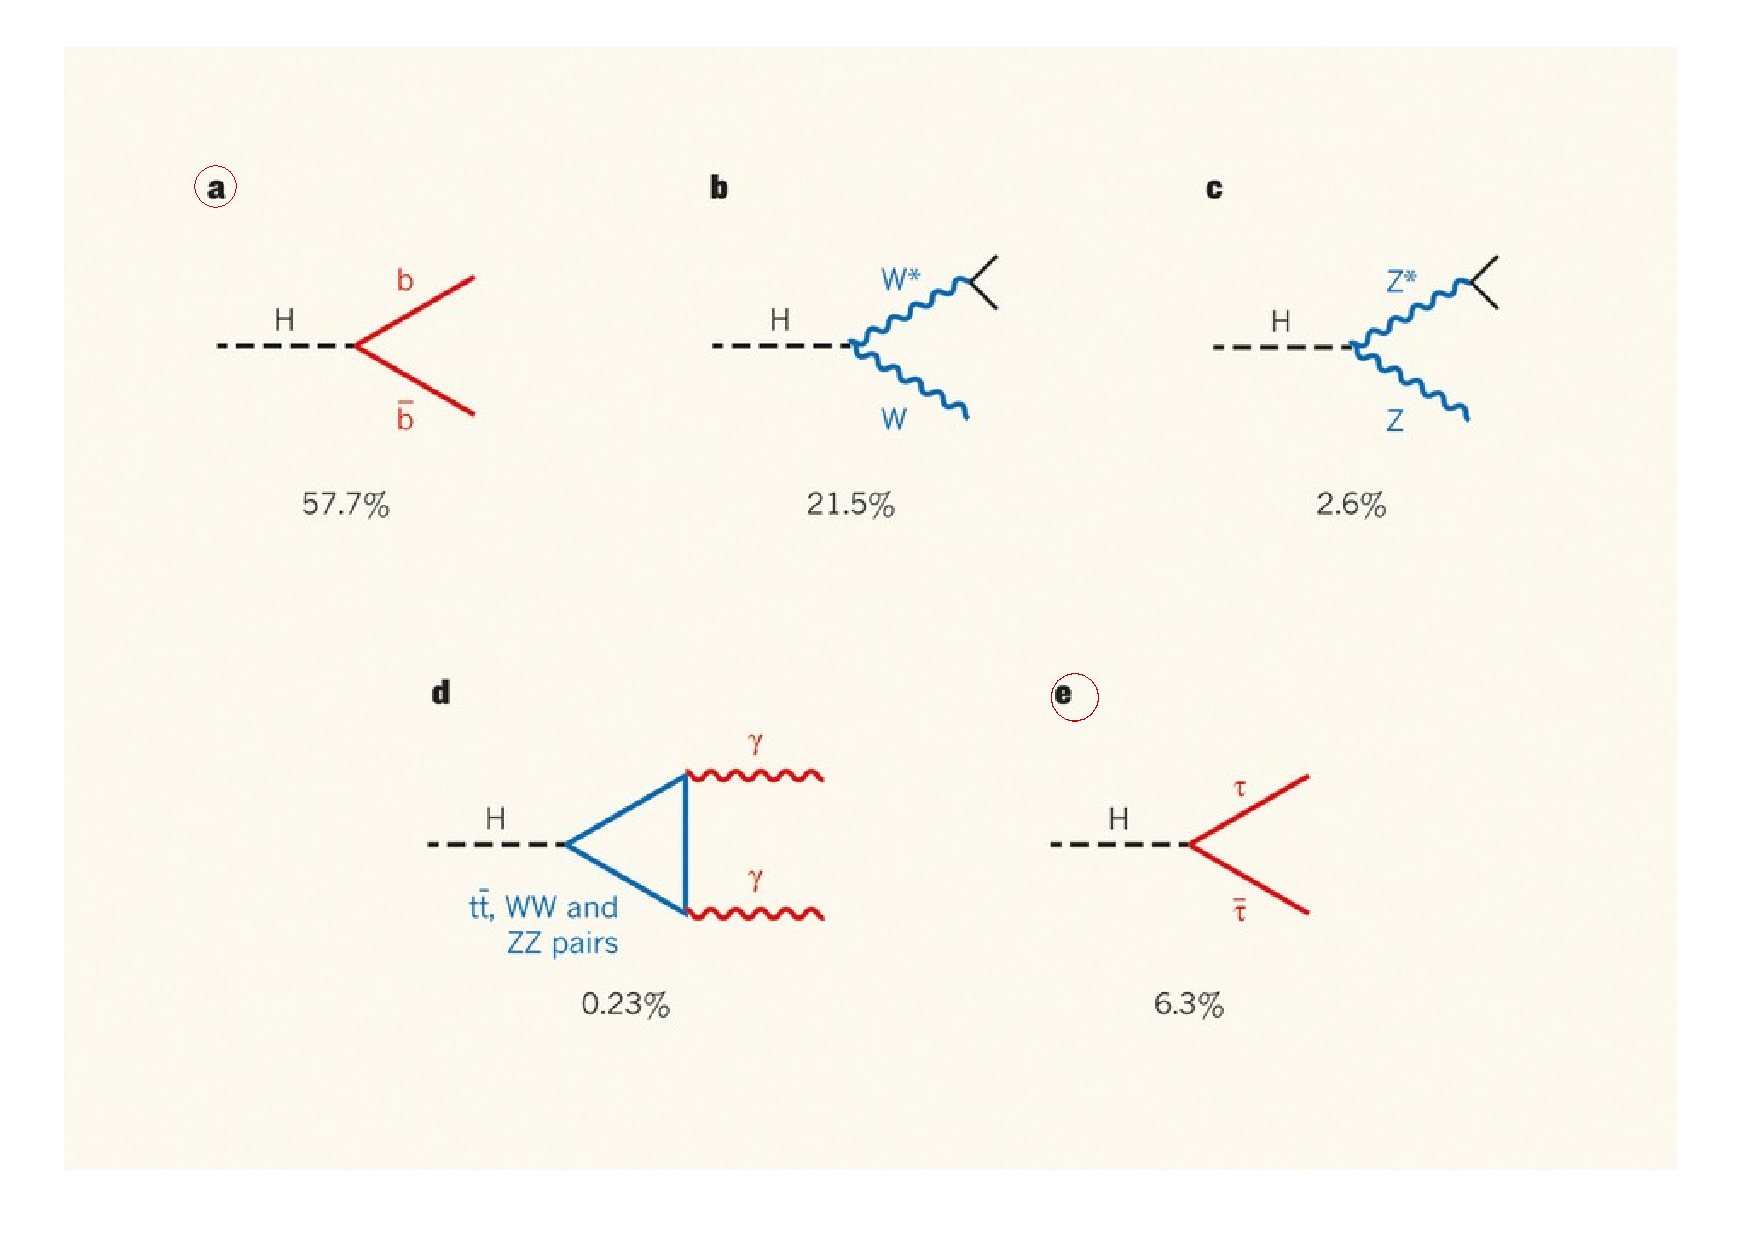
\includegraphics[scale=0.4]{higgs_branching.pdf} 
\end{frame}

\begin{frame}
\frametitle{H $\rightarrow$ $\tau\tau$}
In the original discovery the Higgs was seen decaying into $\gamma\gamma$, $WW$ and $ZZ$. The $H\rightarrow \tau\tau$ channel is particularly interesting as it hasnt been experimentally verified .i.e. the Higgs to tau-tau excess is not yet at
5$\sigma$.
This decay channel is particularly hard to explore due to two reasons:
\begin{itemize}
\item<1-> The decay into two taus is not a unique channel, in fact the Z boson can also decay into two taus, further this happens a lot more frequently than the Higgs. The two decays produce events which have very similar signatures and this prevents a clean separation of the parent candidate.
\item<2-> Taus are heavy and unstable, they decay instantaneously. Their dominant decay modes involve neutrinos and the presence of these undetectable particles in their decay make it difficult to reconstruct the mass of the Higgs on an event by event basis.
\end{itemize}
\end{frame}

\begin{frame}
\frametitle{Decay signatures}
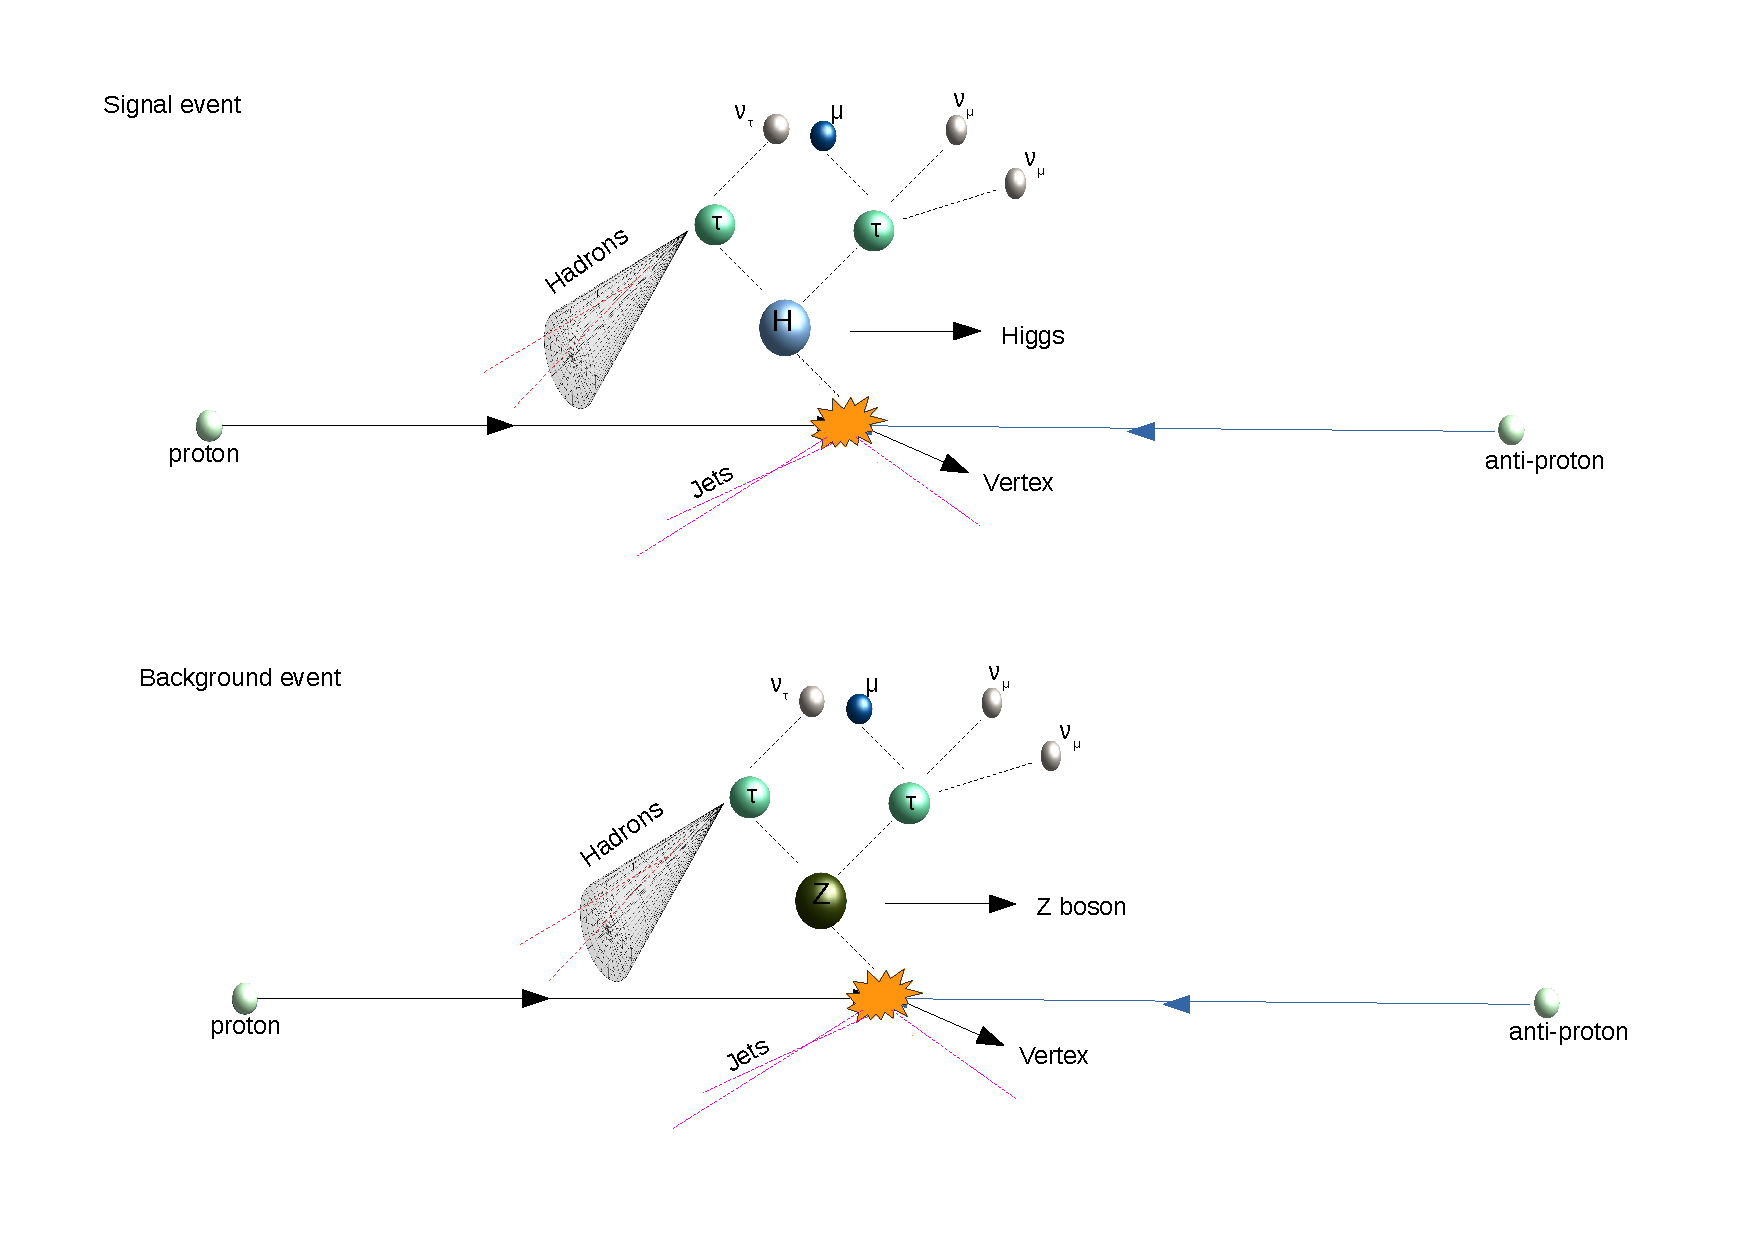
\includegraphics[scale=0.4]{higgs_decay.pdf}
\end{frame}

\begin{frame}
\frametitle{The formal problem}

Inputs : $\mathcal{D} = \{(\mathbf{x}_{1},y_{1},w_{1}),...(\mathbf{x}_{n},y_{n},w_{n}) \}$\\
$\mathbf{x}_{i} \in \mathbb{R}^d,$\\
$y_{i} \in \{b,s\},$\\
$w_{i} \in \mathbb{R}^{+}$ \\
$\mathcal{S} = \{i : y_{i} = s\}$ and $\mathcal{B} = \{i : y_{i} = b\}$\\
$n_{s} = |\mathcal{S}|$ and $n_{b} = |\mathcal{B}|$ 
\begin{equation}
\sum_{i \in \mathcal{S}} w_{i} = N_{s} \hspace{5mm} 
\textrm{ and } \hspace{5mm} 
\sum_{i \in \mathcal{B}} w_{i} = N_{b} 
\end{equation}
The constants have physical meaning, they are the expected total number of signal and background events during the time interval over which the data has been recorded (in the dataset used, it is the year 2012).
\end{frame}

\begin{frame}
\frametitle{The formal statement}
Based on the inputs provided we train a classifier, $h$, generating a selection region, 
$\mathcal{H} = \{\textbf{x} : h(\textbf{x}) = s\}$, $\textbf{x} \in \mathbb{R}^{d}$.\\
$ \hat{\mathcal{H}} = \{i : \textbf{x}_{i} \in \mathcal{H}\}$ is the index set. 

The quantities, 
\begin{equation} 
s = \sum_{i \in \mathcal{S}\cap \hat{\mathcal{H}}} w_{i} \hspace{5mm}
\textrm{    and    } \hspace{5mm}
b =\sum_{i \in \mathcal{B}\cap\hat{\mathcal{H}}} w_{i} 
\end{equation} 
are the true positives and false positives which are used to calculate the AMS = $\dfrac{s}{\sqrt{b}}.$
\end{frame}

\begin{frame}
\frametitle{The Data}
\begin{itemize}
	\item<1-> The ATLAS experiment have made publicly available a simulated (labelled) dataset that has been used by physicists in analysing the Higgs  to tau-tau decay. 
	\begin{enumerate}
	\item Training Set: 250K events
	\item Test Set: 450K events
	\item Validation Set: 100k events
\end{enumerate}	  
	\item<2-> In nature, signal events occur much less frequently than background events. However, the dataset published has been enriched with signal events (30:70) to present a more balanced classification problem. 
	\item<3-> To compensate for this bias, all events
are weighted with importance weights reflecting their probability of occurrence.
\end{itemize}
\end{frame}

\begin{frame}
\frametitle{The machine learning perspective}
\textbf{Goal}:\\

To propose a classifier $h$ to identify a signal-rich region in the feature space where an excess of signal over background events are expected $\bigg(\dfrac{s}{\sqrt{b}}\bigg)$.\\
\bigskip
\textbf{Challenges}:\\
\begin{itemize}
\item The signal and background classes densely overlap.
\item The discovery significance metric the AMS is unusual, noisy. 
\end{itemize}
\end{frame}

\begin{frame}
\frametitle{Class overlap}
\hspace*{-10mm}
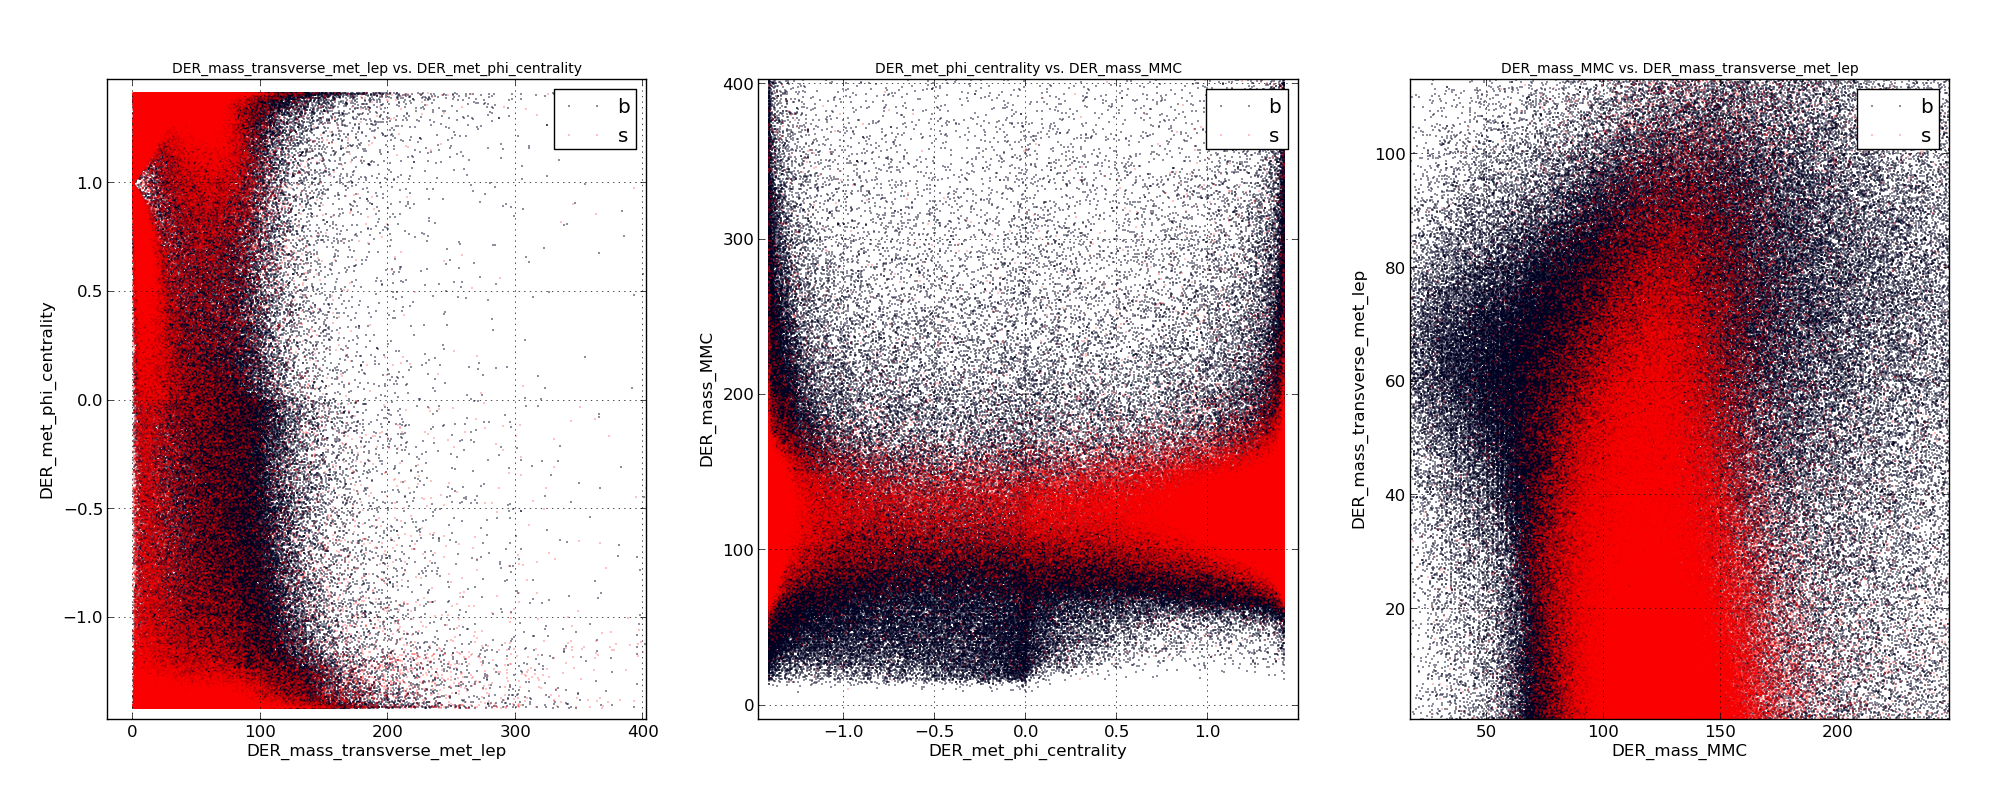
\includegraphics[scale=0.25]{top_bi_features.png}
\end{frame}

\begin{frame}
\frametitle{Class overlap}
\hspace*{-9mm}
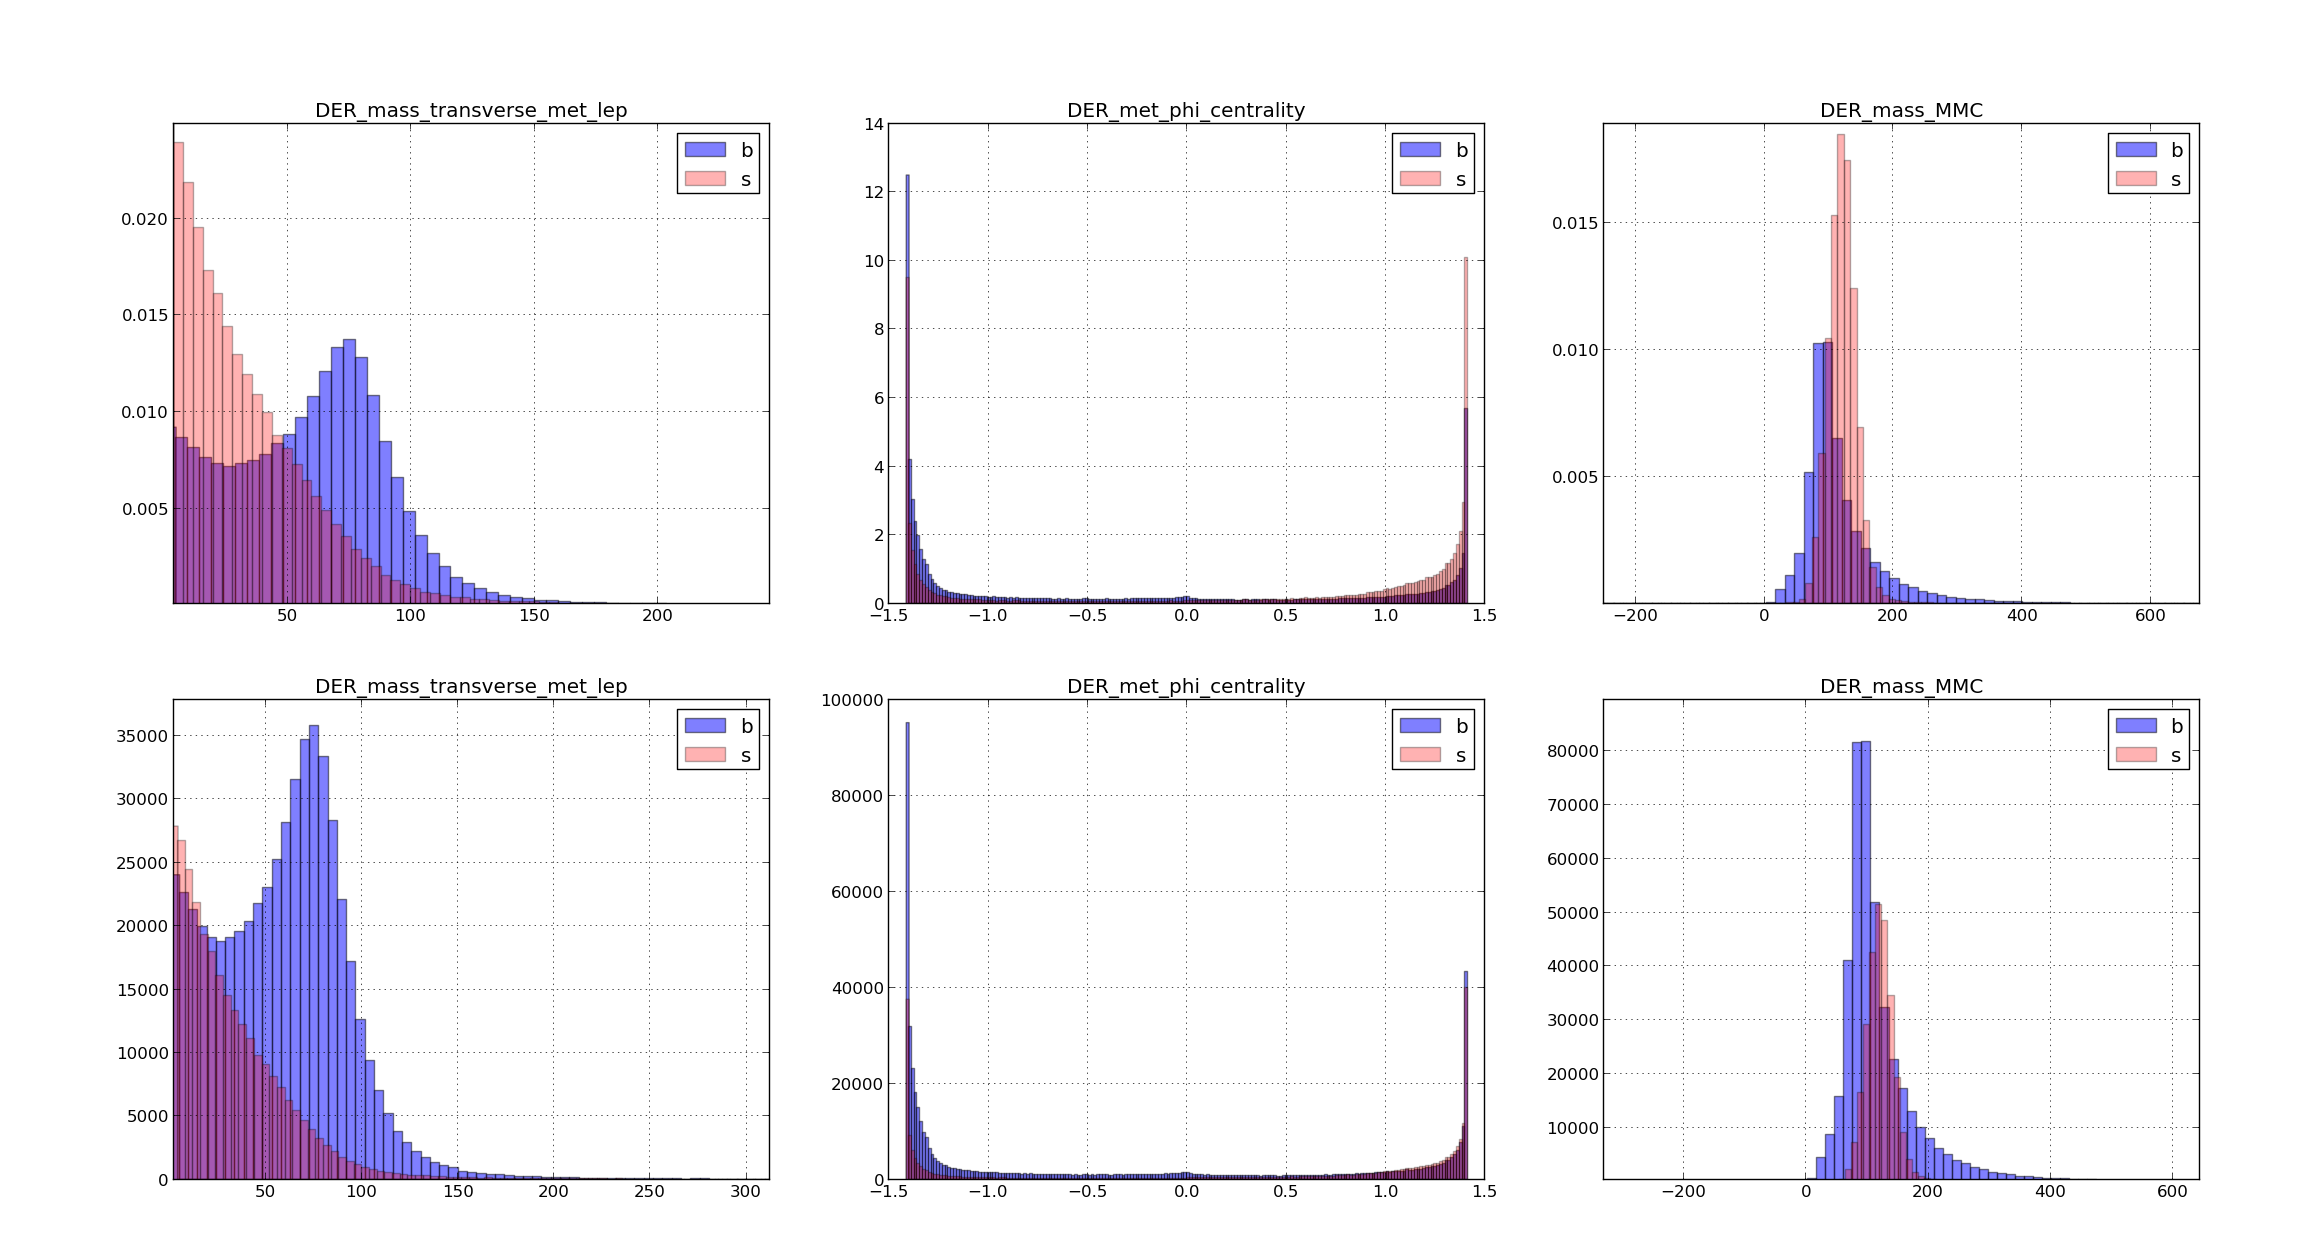
\includegraphics[scale=0.2]{top_hist.png}
\end{frame}

\begin{frame}
\frametitle{Density}
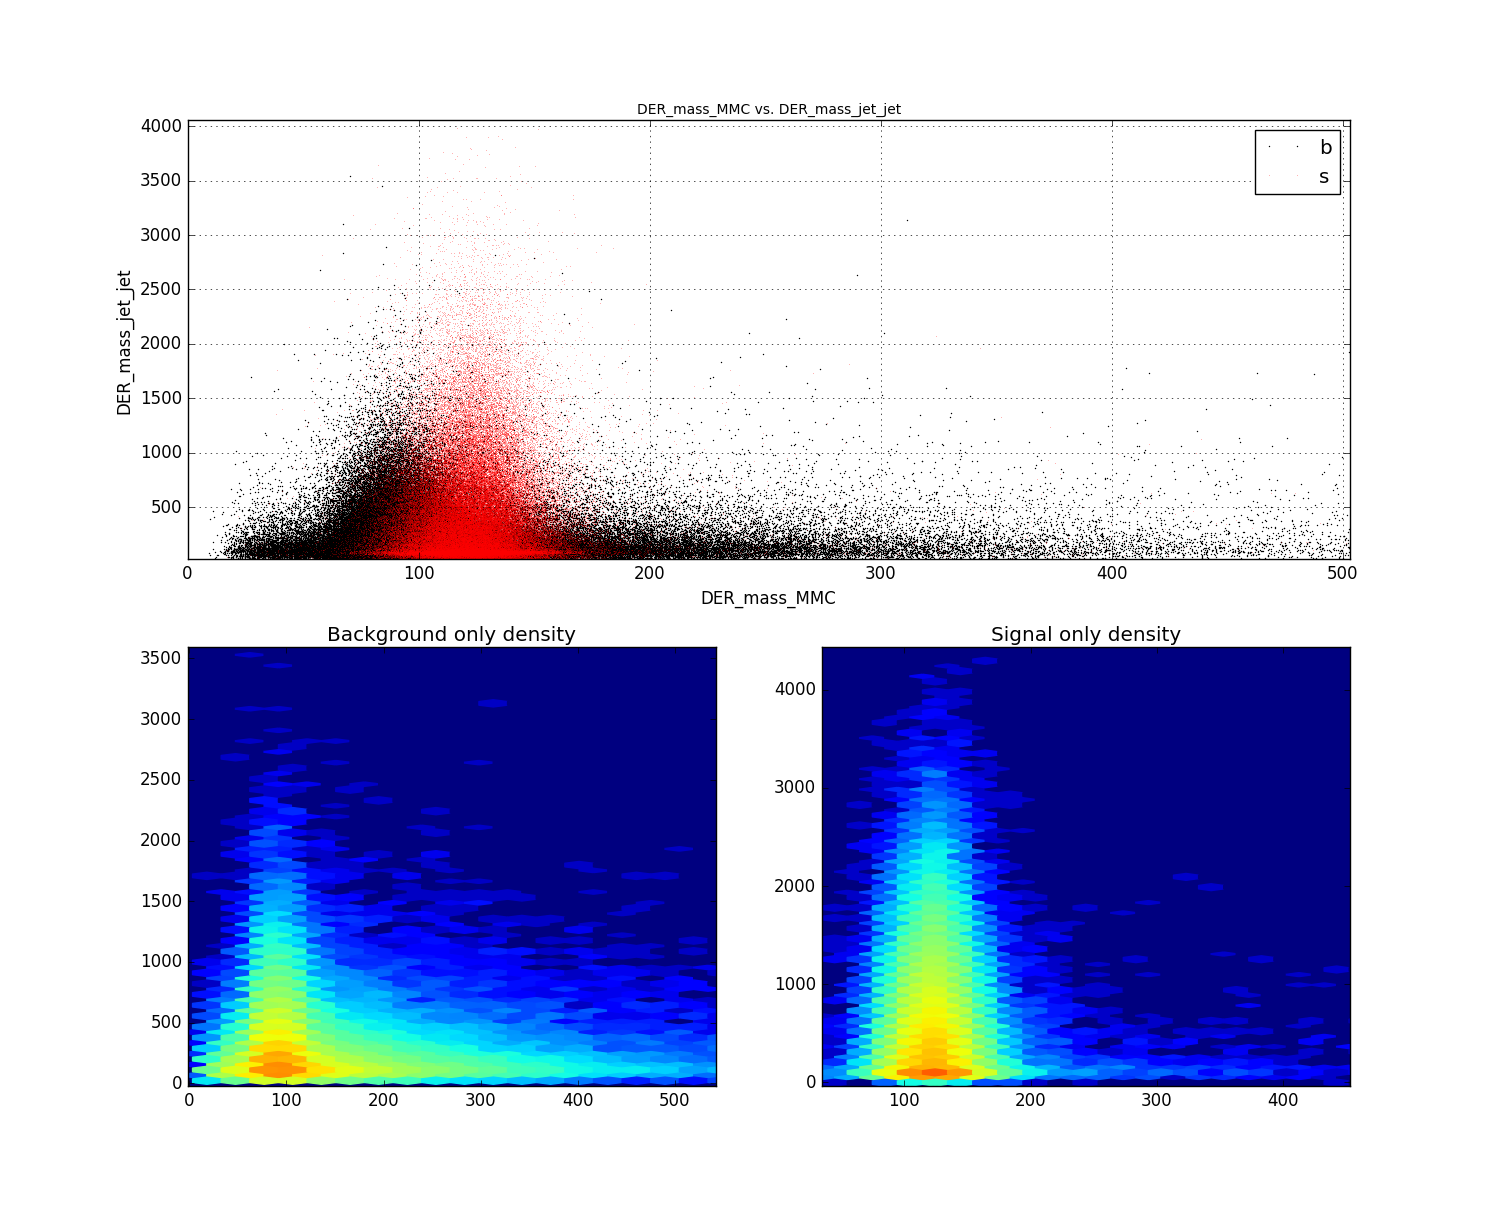
\includegraphics[scale=0.27]{density.png}
\end{frame}

\begin{frame}
\frametitle{Boosting Algorithm}
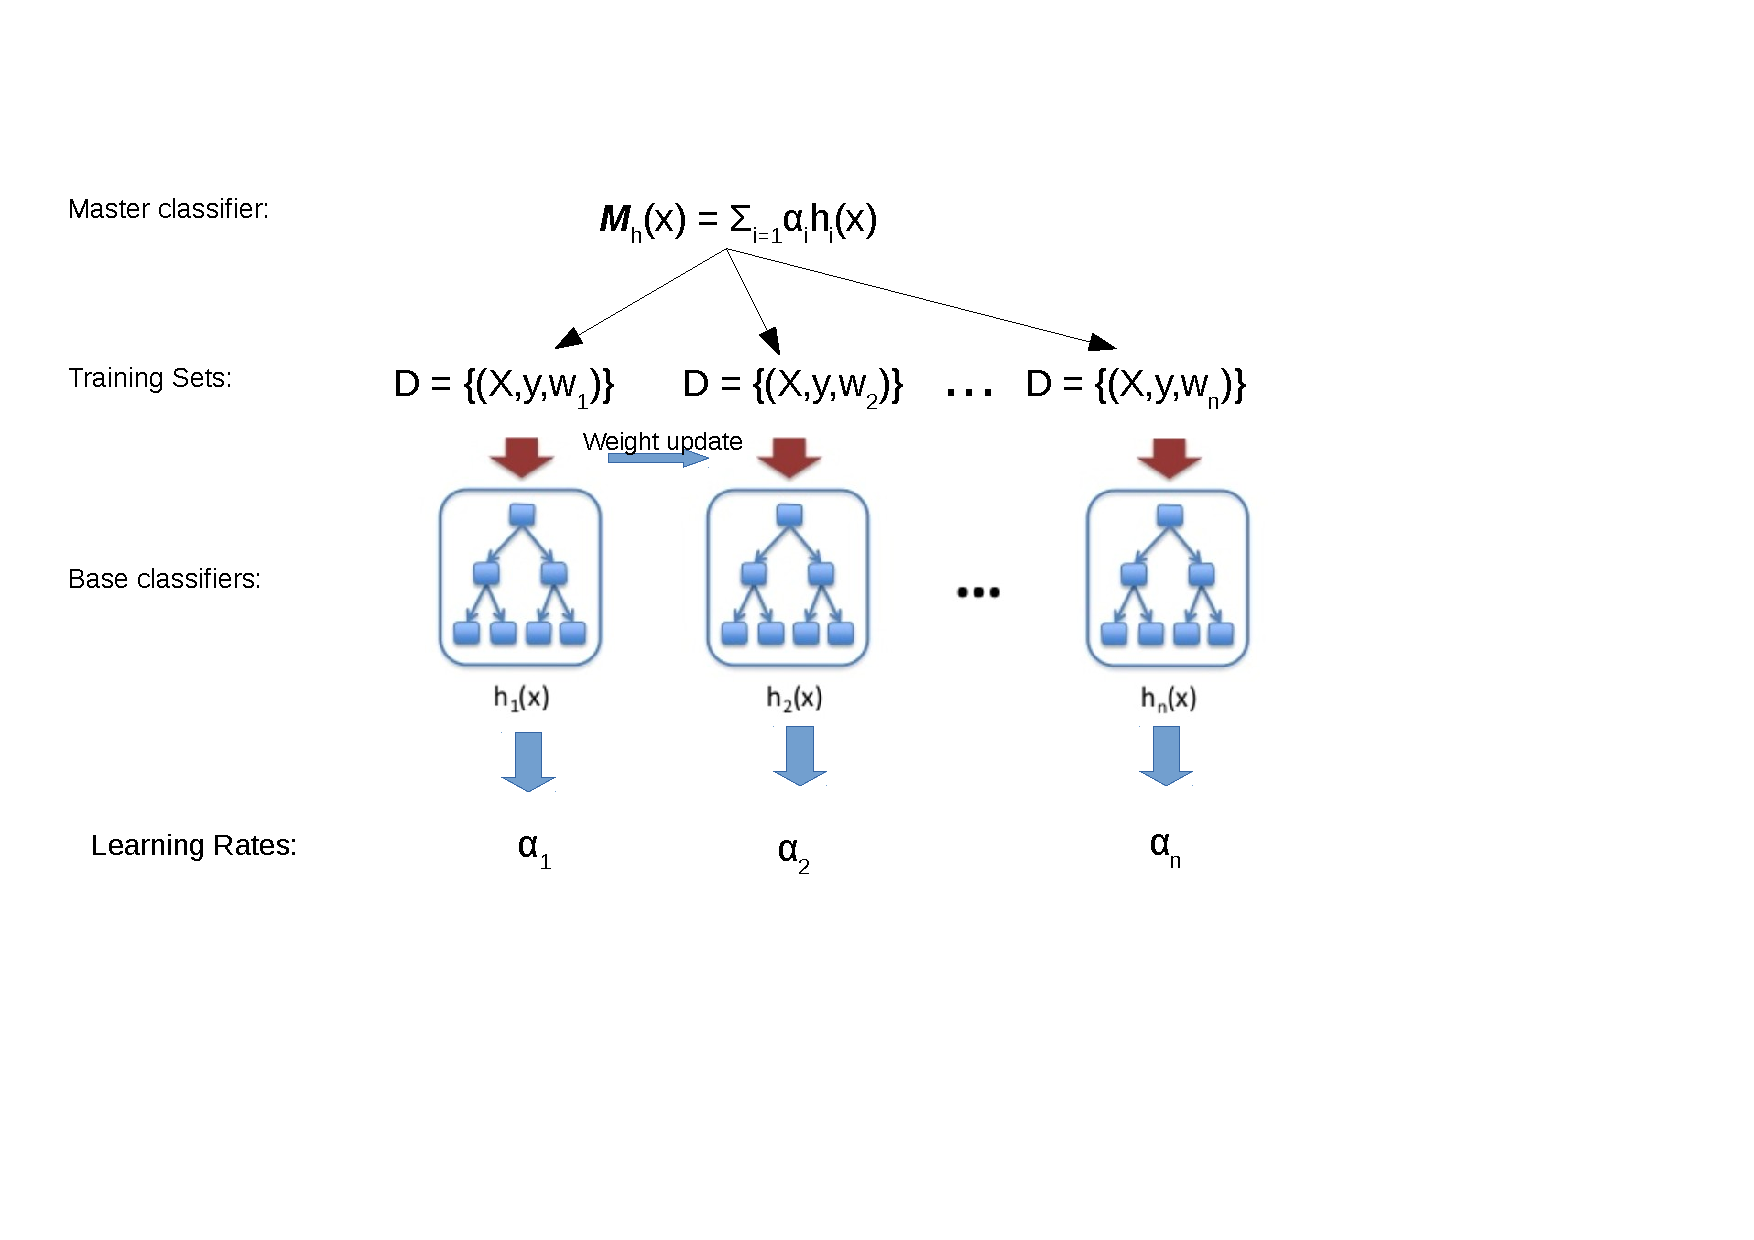
\includegraphics[scale=0.5]{boosting.pdf}
\end{frame}

\begin{frame}
\frametitle{Boosting Algorithm}
\begin{algorithm}[H]
\caption{AdaBoost with $M$ stages}
\begin{algorithmic}[1]
\STATE Initialize the data weighting coefficients $\{ w_{i}\} = 1/N$ $\forall i=1...N$  
\FORALL{$m$ = 1...M} 
\STATE \textbf{Fit} classifier $h_{m}(\mathbf{x})$ by minimizing the weighted error function $R(h_{m}) = \sum_{i=1}^{N}w_{i}\mathbf{I}(h_{m}(\mathbf{x}_{i}) \neq y_{i})$ 
\STATE \textbf{Compute} error rate $\epsilon_{m}$ as the fraction of misclassified samples.
\STATE \textbf{Compute} classifier weight $\alpha_{m} = \dfrac{1}{2}\ln\bigg(\dfrac{1-\epsilon_{m}}{\epsilon_{m}}\bigg)$
\STATE \textbf{Update} weights for stage $(m+1)$ by, $w_{i}^{(m+1)} = w_{i}^{(m)}e^{\alpha_{m}\mathbf{I}(h_{m}(\mathbf{x}_{i}) \neq y_{i})}$ 
\ENDFOR
\STATE $M_{h}(\textbf{x}) = \sum_{m=1}^{M}\alpha_{m}h_{m}(\mathbf{x})$   
\RETURN 
\end{algorithmic}
\label{ada}
\end{algorithm}
\end{frame}

\begin{frame}
\frametitle{Baseline performance}
\begin{center}
\begin{table}[H]
\resizebox{\textwidth}{!}{
\begin{tabular}{l|c|c|c}
\textbf{Classifier} & \textbf{Precision} [TP/(TP+FP)] & \textbf{Recall} [TP/P] & AMS\\
\toprule
\textbf{Weak Learner} & & &\\ 
Background  & 0.79 & 0.79 &\\
Signal & 0.60 &  0.61 & \\
Average & 0.73 & 0.73 & 2.33$\sigma$\\
\midrule
\textbf{AdaBoost with weak learner} & & &\\
Background  & 0.84 & 0.84 &\\
Signal & 0.69 & 0.68  &\\
Average & 0.79 & 0.79 & 2.87$\sigma$\\
\midrule
\textbf{Strong learner} & & &\\
Background  & 0.84 & 0.90 & \\
Signal & 0.76  & 0.62 & \\
Average & 0.80 & 0.80 & 3.41$\sigma$\\
\midrule
\textbf{AdaBoost with strong Learner} & & &\\
Background  & 0.86 & 0.89 & \\
Signal &0.77 & 0.71  &\\
Average & 0.83 & 0.83 & 3.52$\sigma$\\
\midrule
\end{tabular}}
\label{pr}
\end{table}
\end{center}
\end{frame}

\begin{frame}
\frametitle{ROC curves}
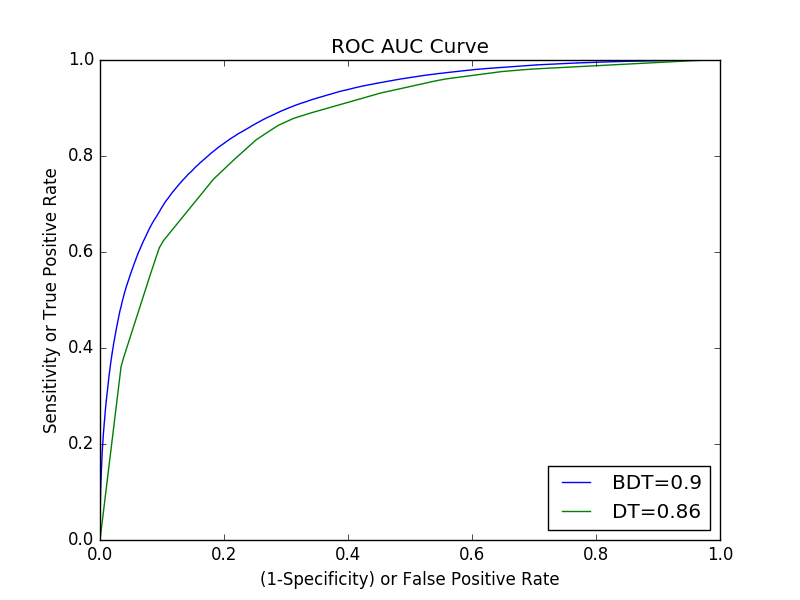
\includegraphics[scale=0.5]{roc.png}
\end{frame}

\begin{frame}
\frametitle{Signal Sensitivity}
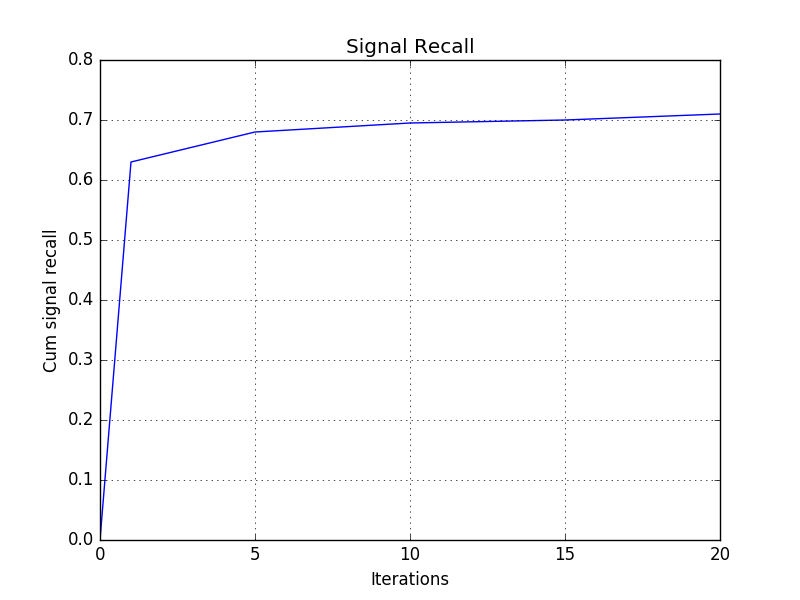
\includegraphics[scale=0.5]{sr.png}
\end{frame}

\begin{frame}
\frametitle{The \textit{meta} approach}
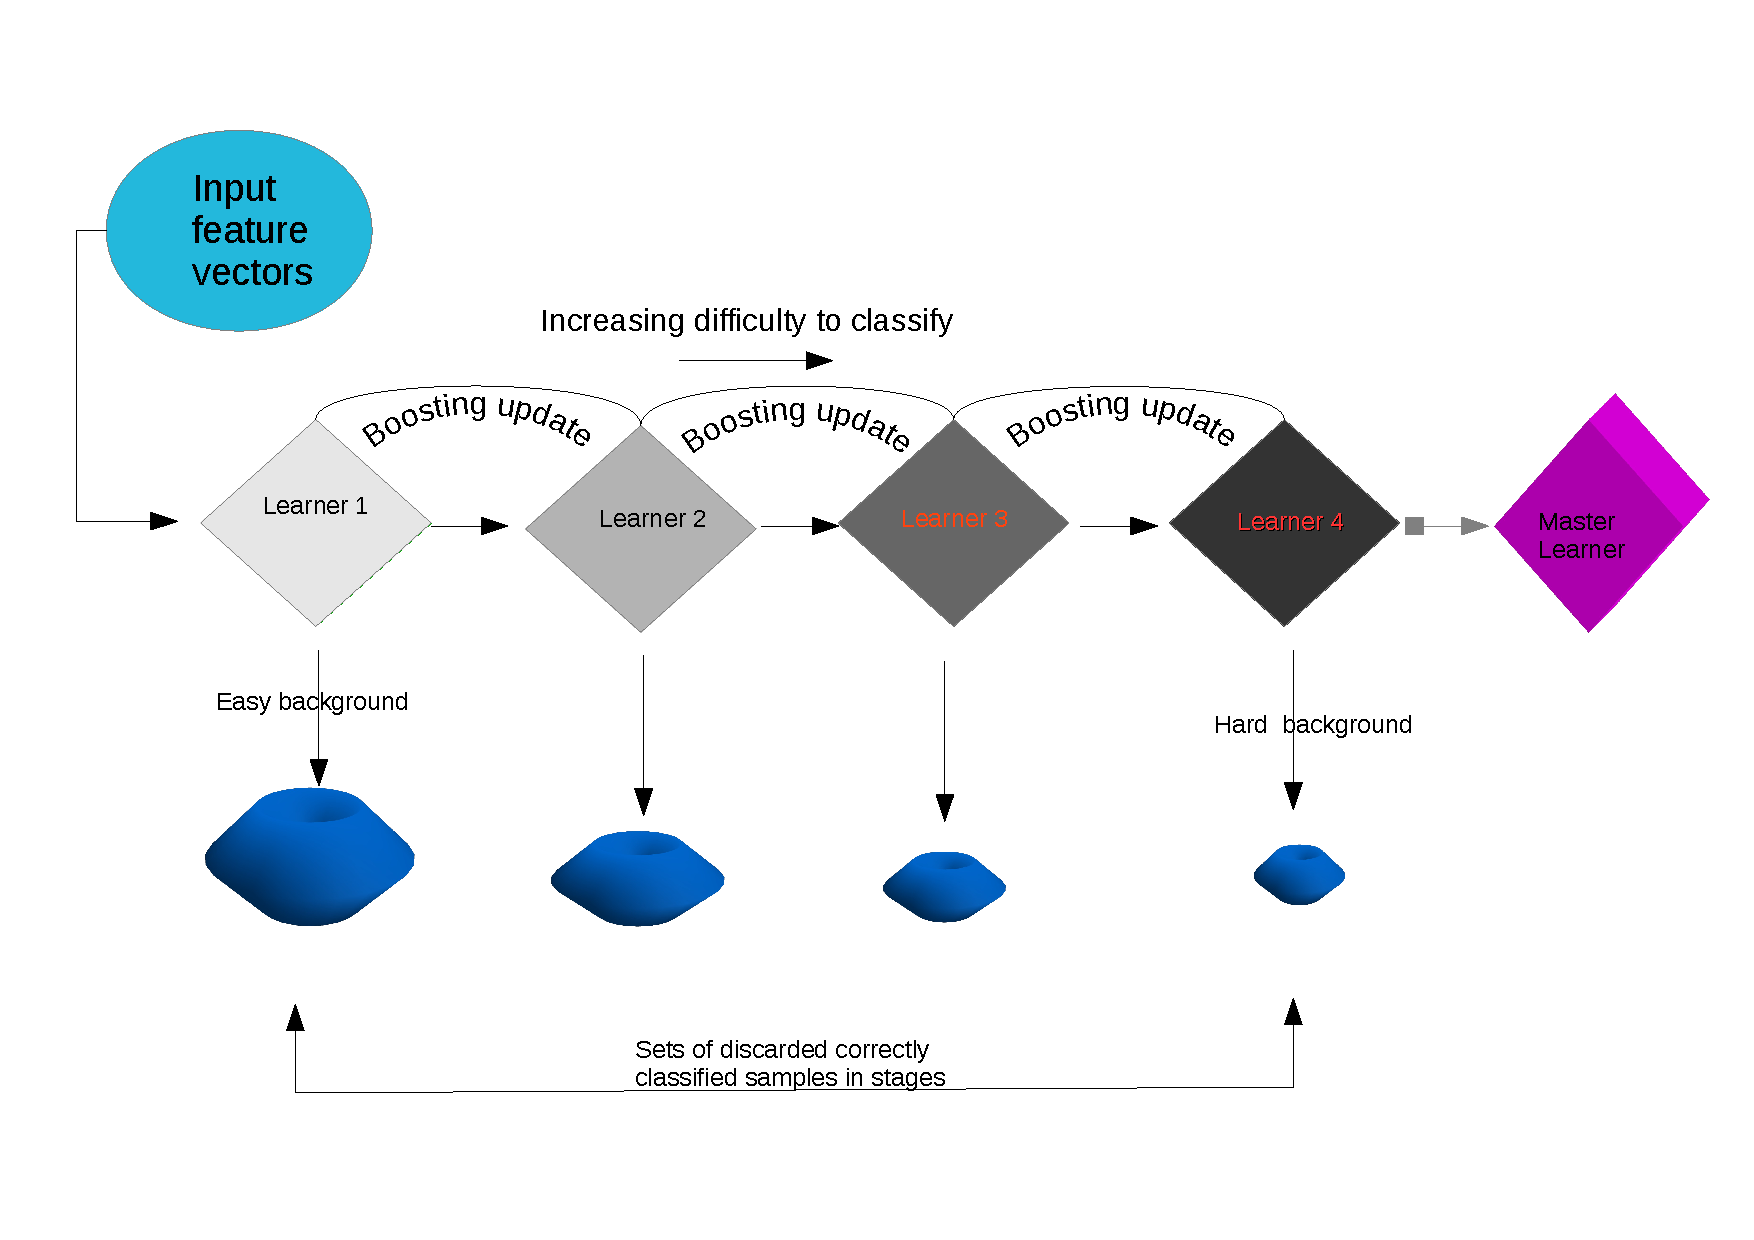
\includegraphics[scale=0.4]{MB.pdf}
\end{frame}

\begin{frame}
\frametitle{Fragmenting the feature space}
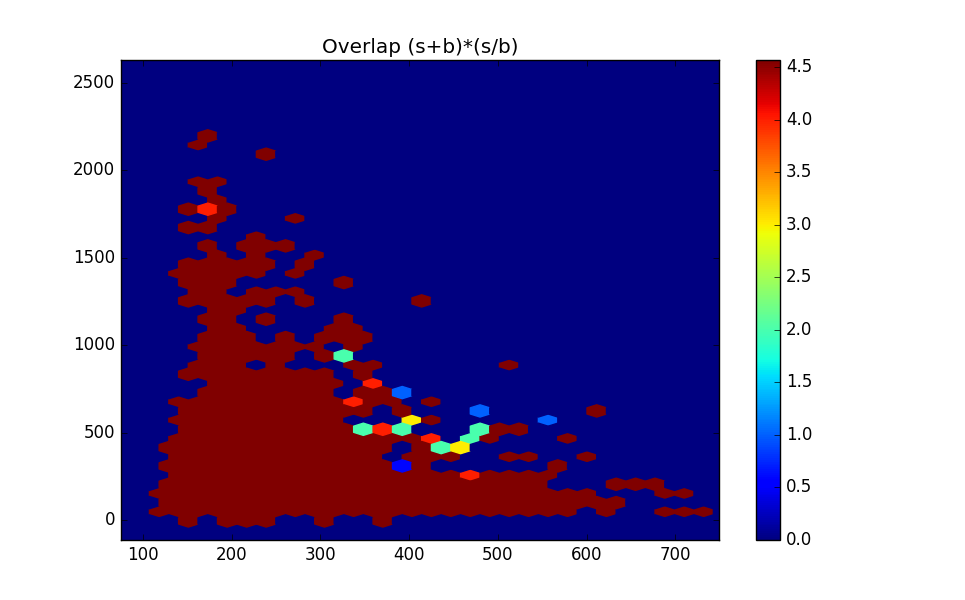
\includegraphics[scale=0.4]{overlap.png}
\end{frame}

\begin{frame}
\frametitle{Targets for Algorithm Design}
\begin{itemize}
\item Adaptive selection of features.
\item Diversity in component classifiers of the ensemble. 
\item Targetting overlapping regions during training. 
\item Focus on improving signal sensitivity $\Rightarrow$ maximixing AMS.
\end{itemize}
\end{frame}

\begin{frame}{Open problems}
\begin{itemize}
\item Control for overfitting/overtraining (bias-variance trade-off). 
\item The choice of component classifiers at each stage of the classification.
\item Demonstrate usage on datasets outside of a HEP context that demonstrate class overlap. 
\end{itemize}
\end{frame}

\begin{frame}
\frametitle{Application Domains}
The main contribution of this work is to develop an algorithm that is generally applicable in domains where the data sets exhibit the problem of class-overlap in binary or multiple-classes. \\
\begin{itemize}
\item{Medical Diagnosis}
\item{Fraud detection}
\item{Psychiatry (predicting criminality potential in individuals)}
\item{Loan default predictions}
\item{Geochemical distributions}
\end{itemize}
\end{frame}

\begin{frame}
\frametitle{Timeline}
\hspace*{-6mm}
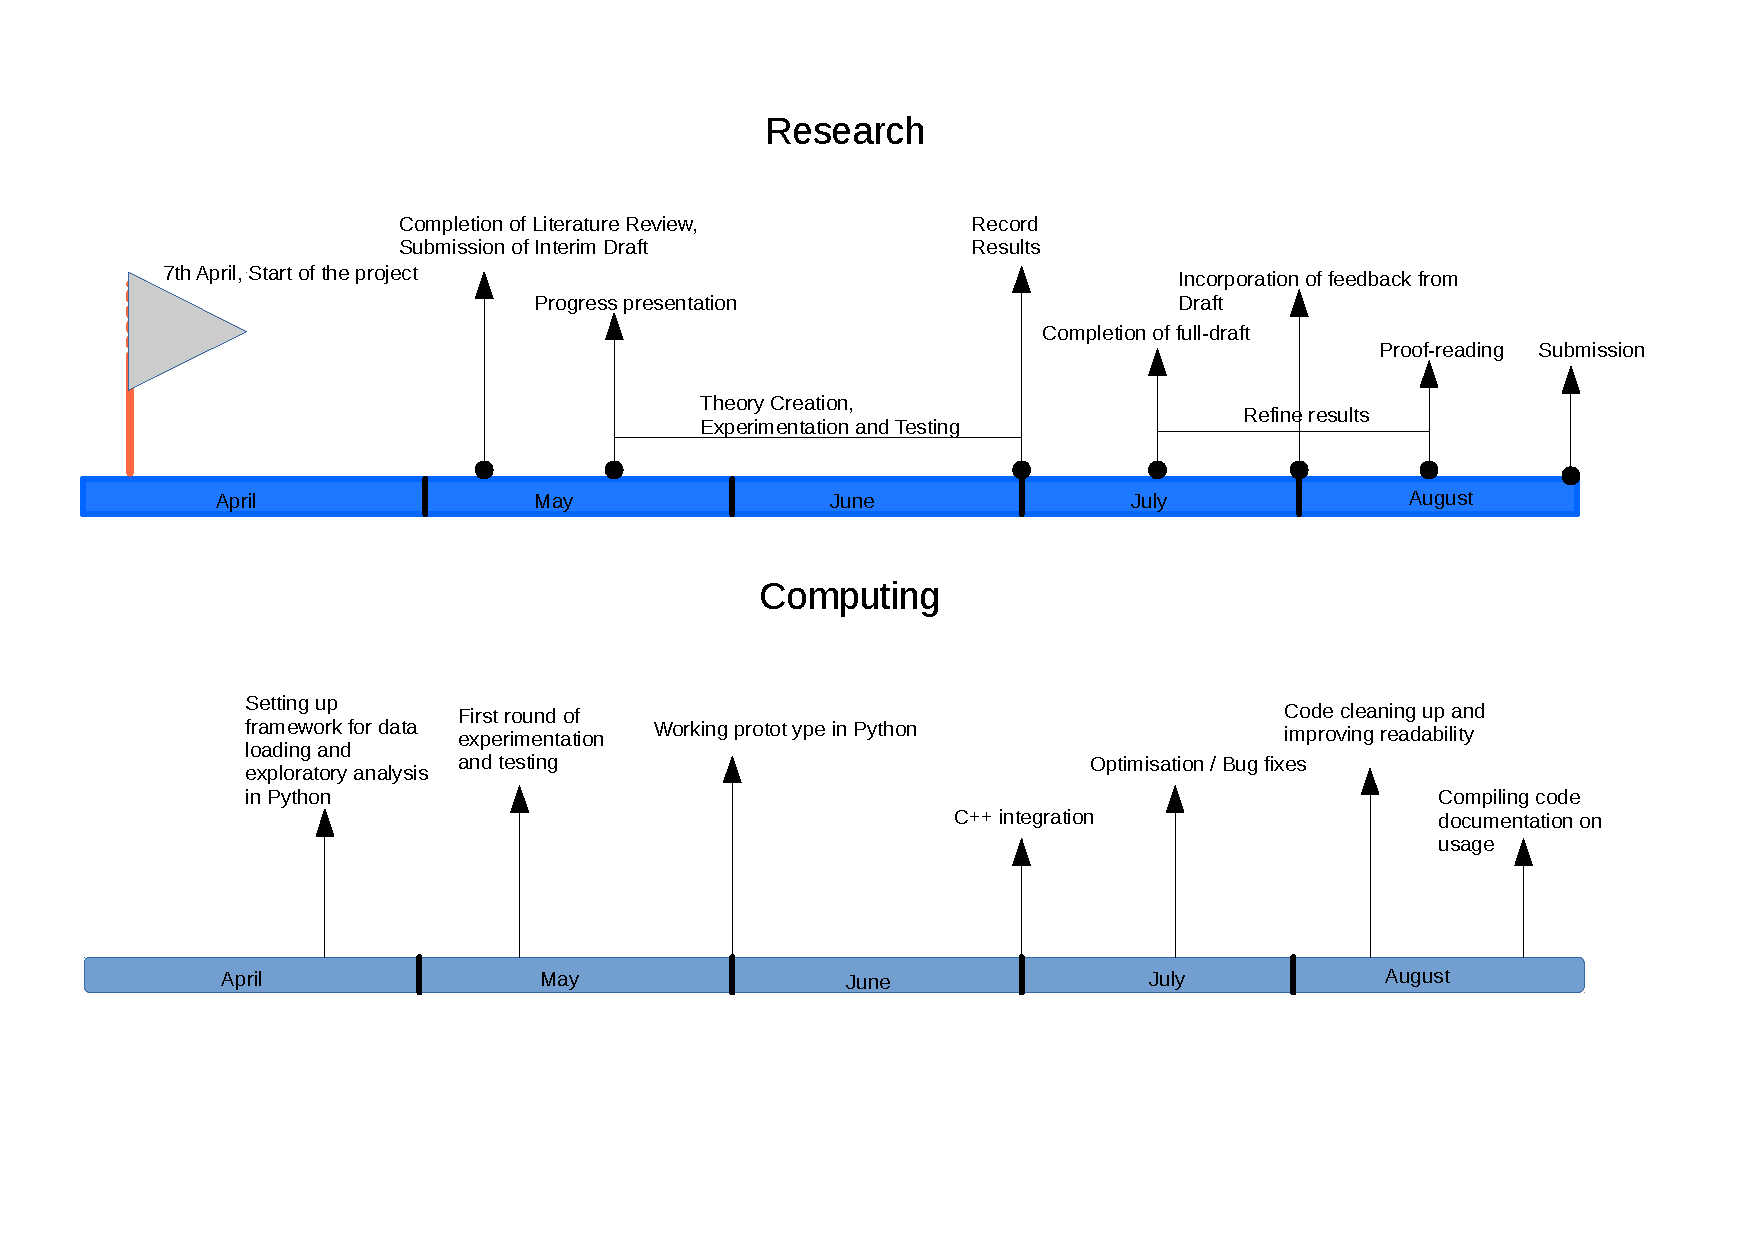
\includegraphics[scale=0.41]{timeline.pdf}
\end{frame}

\begin{frame}
\frametitle{Critical references}

\begin{thebibliography}{t}
\bibitem[HiggsML, 2014]{Ref}
Journal of Machine learning Research, Workshop and Conference Proceedings 42:19-55, 2015
\newblock {\em The Higgs Boson Machine learning challenge}
\newblock {\tt http://jmlr.org/proceedings/papers/v42/cowa14.pdf}

\bibitem[bt]{bt}
ACM Transactions on Embedded Computing Systems, Vol. 9, No. 4, Article 1, April 2015
\newblock {\em A Review of Boosted Machine learning Techniques for Particle Identification at ALICE}
\newblock {\tt https://people.cs.uct.ac.za/~wngrya001/\\
documentation/lit$\_$review$\_$particle$\_$identify.pdf}

\end{thebibliography}
\end{frame}

\begin{frame}
\frametitle{TensorFlow Library}
\begin{center}

\includegraphics[scale=0.3]{skflow.jpg}
\end{center}
\begin{itemize}
\item Google's \textbf{\textit{TensorFlow}} is an open source application grade machine learning library written in Python and C++ with full API support.
\item It offers deep learning models on a flexible architecture and is accessible through a python API and a lesser documented C++ API.   
\item CERN has expressed interest in using TensorFlow technology for machine learning tasks in the realm of HEP. 
\item TensorFlow can run on multiple CPUs and GPUs with optional CUDA extensions. 
\item It was developed by Dr. Geoffrey Hinton and Dr. Jeff Dean.
\end{itemize}
\end{frame}


\begin{frame}
\begin{center}
- Thank you -\\
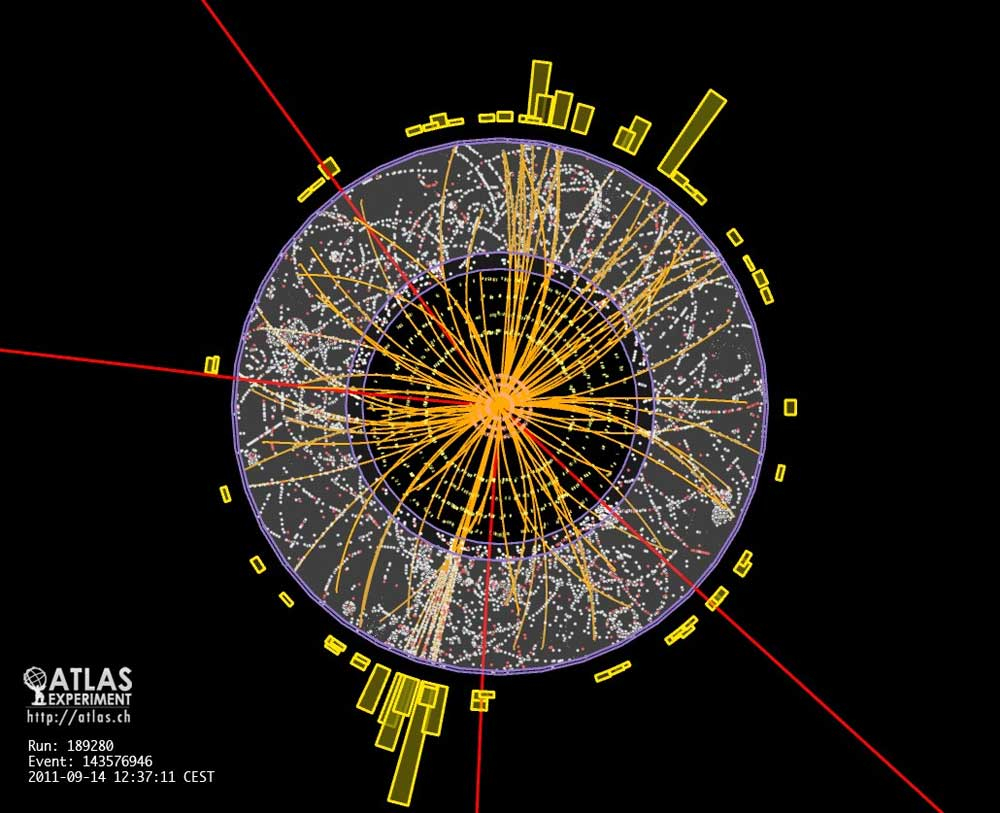
\includegraphics[scale=0.2]{lhc-atlas-protons.jpg}\\
\end{center}
\end{frame}

\end{document}
